\chapter{Resultados}
\label{chap:result}
Nesta seção serão demonstrados os trabalhos realizados durante o período do curso de formação em Robótica e Sistemas Autônomos, identificando nos apêndices os relatórios, mapas mentais e apresentações realizadas. E nos textos são indicados os repositórios onde é possível verificar os códigos, os pré-requisitos para funcionar o pacote e o tutorial para realizar a simulação ou o modelo real.

%--------- NEW SECTION ----------------------
%\section{Programação do \textit{Turtlesim} no \textit{ROS} em \textit{Python}}
%\label{sec:testu}
%Como mencionado anteriormente, nas primeiras semanas foram inicializadas as atividades dentro da programação do curso onde neste primeiro momento começamos a etapa de absorção e desenvolvimento de conhecimentos que nos seriam requeridos durante todo o curso.
%No repositório \url{https://github.com/JessMotta/desafio_turtlesim_setpoint} encontra-se a primeira atividade desenvolvida, onde foi realizada a programação do \textit{Turtlesim}, no  \textit{ROS}, na linguagem de programação \textit{Python}. Este desafio teve por finalidade inicializar o contato com o \textit{ROS}, pois esse \textit{framework} é o mais utilizado na robótica, e a linguagem de programação \textit{Python} também é uma das mais utilizadas nessa área.
%O desafio constituia realizar a programação do \textit{Turtlesim} para que ele se movimentasse para locais específicos definidos pelo usuário.

%\section{Aprendizado do \textit{OpenCV}}
%\label{sec:intsis}
%O \textit{OpenCV (Open Source Computer Vision)} é uma biblioteca de código aberto que tem por finalidade tornar mais acessível para desenvolvedores a visão computacional. Nesse repositório \url{https://github.com/JessMotta/opencv_learning} é possível encontrar o código estruturado em \textit{Python} e os conhecimentos obtidos no primeiro contato com \textit{OpenCV} e suas possibilidades de aplicação. Além do que nos foi orientado que essa biblioteca seria muito utilizada para os projetos que iríamos desenvolver na área de robótica e sistemas autônomos. 

%--------- NEW SECTION ----------------------
\section{Desafio 1.0 }
\label{sec:desafio_1}
O primeiro desafio, disponível no repositório \url{https://github.com/JessMotta/challenge_ws}, nele é possível verificar os pré-requisitos e o que é necessário para executar a simulação. Este desafio foi feito individualmente, e ele foi realizado com o objetivo de programar o robô da \textit{Clearpath Robotics- Husky}, no ambiente de simulação do \textit{Gazebo}. A área de operação desse robô foi a área externa entre os prédios do CIMATEC 3 e 4, como mostrado na Figura \ref{fig:cimatec3_4}. O \textit{Husky} tinha como missão explorar esse ambiente externo a procura de uma bola amarela, e ao identificar esta ele deveria ir até ela e parar de frente para mesma informando que a missão foi completada.  


\begin{figure}[H]
    \caption{Área externa do CIMATEC 3 e 4, ambiente de simulação do \textit{Gazebo}}
    \centering
    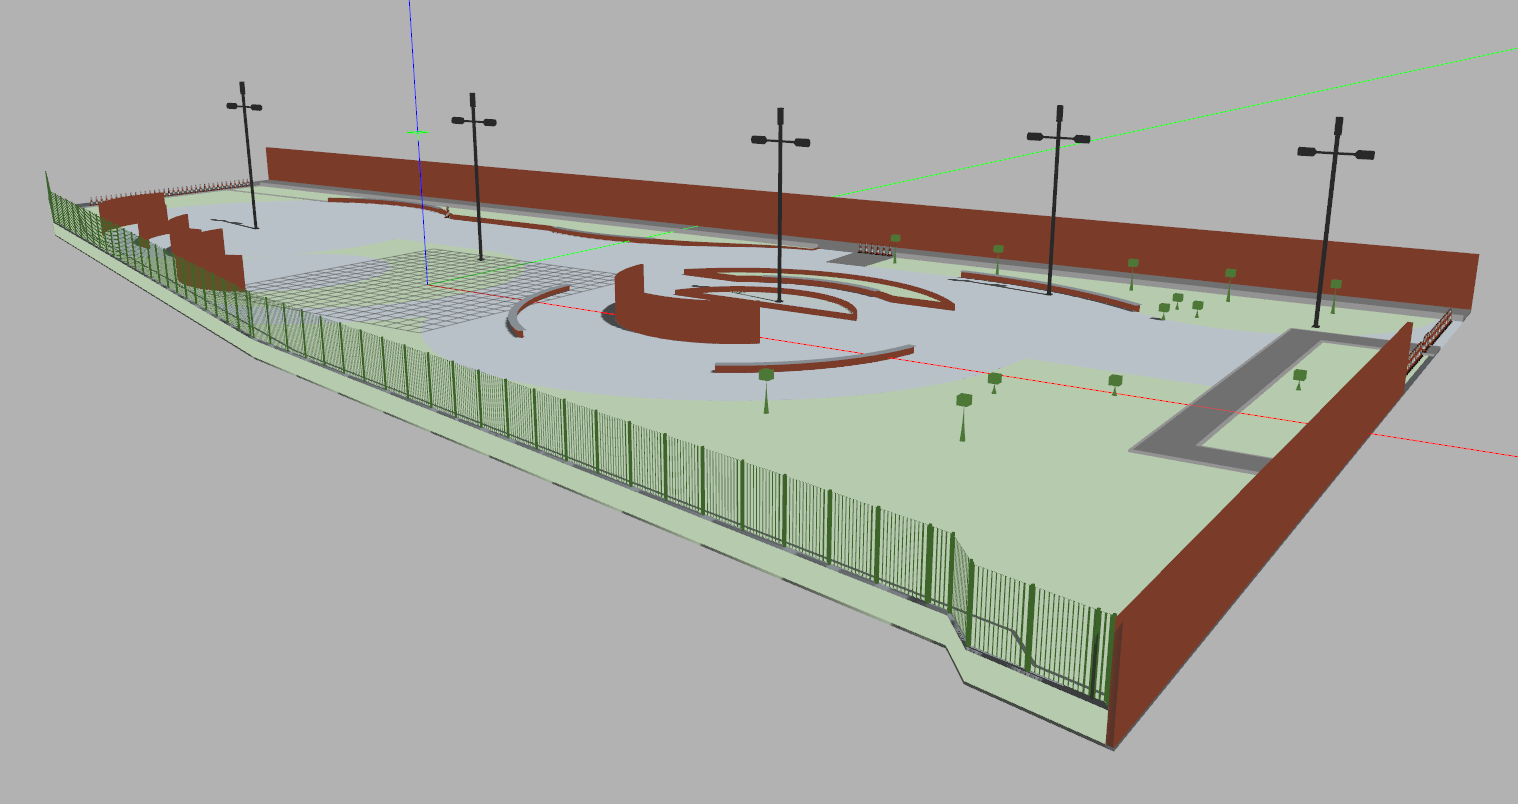
\includegraphics[width= \textwidth]{Figures/cimatec4.png}
    \caption*{Fonte: Grupo de Formação em Robótica e Sistemas Autônomos}
    \label{fig:cimatec3_4}
\end{figure}



\section{Desafio 2.0 }
\label{sec:desafio_2}
O segundo desafio, disponível no repositório \url{https://github.com/Brazilian-Institute-of-Robotics/timon\_hm\_manipulator}, onde neste também tem os pré-requisitos e o tutorial de como executar a simulação. Foi um desafio realizado em grupo composto por mim, Jean, Leonardo, Miguel, Vinícius e Rodrigo, onde um manipulador deveria ser concebido desde sua fase inicial projetando toda sua estrutura e realizada a simulação dele no \textit{Gazebo}, com a missão da câmera integrada ao manipulador identificar o \textit{ArUco} na caixa e pressionar o botão. No apêndice encontra-se o relatório elaborado

\begin{figure}[H]
    \caption{Área externa do CIMATEC 3 e 4, ambiente de simulação do \textit{Gazebo}}
    \centering
    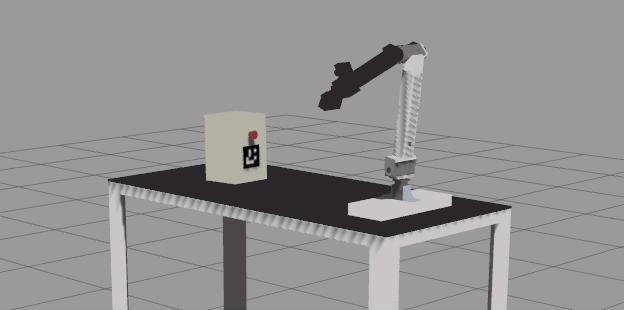
\includegraphics[width= \textwidth]{Figures/manipulador_simulacao.png}
    \caption*{Fonte: Grupo de Formação em Robótica e Sistemas Autônomos}
    \label{fig:manipulador_simulacao}
\end{figure}
